\UseRawInputEncoding
\documentclass[12pt]{article}
\title{ECE C143A Homework 4}
\usepackage{subcaption}
\author{Lawrence Liu}
\usepackage{graphicx}
\usepackage{amsmath}
\usepackage{bm}
\usepackage{pdfpages}
\newcommand{\Laplace}{\mathscr{L}}
\setlength{\parskip}{\baselineskip}%
\setlength{\parindent}{0pt}%
\usepackage{xcolor}
\usepackage{listings}
\definecolor{backcolour}{rgb}{0.95,0.95,0.92}
\usepackage{amssymb}
\lstdefinestyle{mystyle}{
    backgroundcolor=\color{backcolour}}
\lstset{style=mystyle}

\begin{document}
\maketitle
\section*{Problem 1}
\subsection*{(a)}
$P(N=0)=1-0.25=\boxed{0.75}$
\subsection*{(b)}
We want $P(N=0|R=0)$, we know that
$$P(R=1|N=0)=P(E=0)P(R=1|E=0,N=0)+P(E=1)P(R=1|E=1,N=0)=0.01$$
$P(R=0|N=0)=0.99$ and thus from bayes law we have 
\begin{align*}
    P(N=0|R=0)&=P(R=0|N=0)\frac{P(N=0)}{P(R=0)}\\
    &=0.9\frac{0.1\cdot 0.75}{P(R=0)}
\end{align*}
To find $P(R=0)$ we must find $P(R=1)$,
\begin{multline*}
    P(R=1)=P(E=1)P(N=1)P(R=1|E=1,N=1)\\+P(E=1)P(N=0)P(R=1|E=1,N=0)
    \\+P(E=0)P(N=1)P(R=1|E=0,N=1)\\+P(E=0)P(N=0)P(R=1|E=0,N=0)
\end{multline*}
\begin{multline*}
    P(R=1)=0.9\cdot0.25\cdot 1+0.1\cdot0.75\cdot0.1+0.1\cdot 0.25\cdot 0.1=0.235
\end{multline*}
Therefore $P(R=0)=1-P(R=1)=0.765$, thus
$$P(N=0|R=0)=0.99\frac{0.75}{P(R=0)}=\boxed{0.97}$$
\subsection*{(c)}
We have
\begin{align*}
    P(N=0|R=0,E=0)&=\frac{P(E=0,N=0,R=0)} {P(R=0,E=0)}\\
    &=\frac{P(R=0|E=0,N=0)P(E=0,N=0)} {P(R=0,E=0)}\\
    &=\frac{(1-P(R=1|E=0,N=0))P(E=0)P(N=0)} {P(R=0|E=0)P(E=0)}\\
    &=\frac{(1-P(R=1|E=0,N=0))P(N=0)} {(P(R=0|E=0,N=0)P(N=0)+P(R=0|E=0,N=1)P(N=1))}\\
    &=\frac{0.9\cdot 0.75}{0.9\cdot 0.75+0.9\cdot 0.25}\\
    &=\boxed{0.75}
\end{align*}
This intuitively makes sense because the equiment being broken means that a recorded spike provides no aditional information.
\subsection*{(d)}
Let us consider the case $E=1$, $N=0$ given $R=1$ we have
$$P(E=1,N=0|R=1)=\frac{P(R=1|E=1,N=0)P(E=1)P(N=0)}{P(R=1)}$$
Since $P(R=1|E=1,N=0)=0$, we thus have $P(E=1,N=0|R=1)=0$. However 
\begin{align*}
    P(E=1|R=1)&=P(R=1|E=1)\frac{P(E=1)}{P(R=1)}\\
    &=(P(R=1|E=1,N=0)P(N=0)+\\
    &P(R=1|E=1,N=1)P(N=1))\frac{P(E=1)}{P(R=1)}
\end{align*}
This therefore $P(E=1|R=1)>1$, likewise
\begin{align*}
    P(N=0|R=1)&=P(R=1|N=0)\frac{P(N=0)}{P(R=1)}\\
    &=(P(R=1|E=1,N=0)P(E=1)+\\
    &P(R=1|E=0,N=0)P(E=0))\frac{P(N=0)}{P(R=1)}
\end{align*}
This therefore $P(E=1|R=1)>1$, therfore, $P(E=1|R=1)P(N=0|R=1)>0$ and is not equal to $P(E=1,N=0|R=1)$ therefore they are conditionally dependent.
Ie they are not independent given R
\section*{Problem 2}
\subsection*{(a)}
$$\boxed{P(a,b,c,d)=P(c)P(a|c)P(d)P(b|a,d)}$$
\subsection*{(b)}
\begin{align*}
    P(C,D)&=\sum_{A}\sum_{B}P(C,D,A,B)\\
    &=\sum_{A}\sum_{B}P(C)P(D)P(A|C)P(B|A,D)\\
    &=P(C)P(D)\sum_{A}\sum_{B}P(A|C)P(B|A,D)\\
    &=P(C)P(D)\sum_{A}P(A|C)\sum_{B}P(B|A)\\
    &=P(C)P(D)
\end{align*}
Therefore $C$ and $D$ are independent.
\subsection*{(c)}
\begin{align*}
    P(C,D|A,B)&=\frac{P(C,D,A,B)}{P(A,B)}\\
    &=\frac{P(C)P(D)P(A|C)P(B|A,D)}{P(A,B)}\\
    &=\frac{P(C)P(D)P(A|C)P(B,A,D)}{P(A,B)P(A,D)}\\
    &=\frac{P(C)P(D)P(A|C)P(D|B,A)}{P(A,D)}\\
    &=\frac{P(C)P(A|C)P(D|B,A)}{P(A)}\\
    &=P(C|A)P(D|B,A)
    &=P(C|B,A)P(D|B,A)
\end{align*}
Therefore $C$ and $D$ are independent given A and B.
\subsection*{(d)}
\begin{align*}
   P(a,d)&= \sum_{B}P(a,d,b)\\
   &=\sum_{a}P(d)P(b)P(b|d,a)\\
   &=P(d)P(b)\sum_{B}P(b|d,a)\\
   &=P(d)P(b)
\end{align*}
Therefore $a$ and $d$ are independent
\subsection*{(e)}
\begin{align*}
    P(a,d|b)&= \frac{P(a,d,b)}{P(b)}\\
    &=\frac{P(a)P(d)P(b|a,d)}{P(b)}\\
    &=\frac{P(a)P(d)}{P(b)}\frac{P(b|d)P(a|b,d)}{P(a|d)}\\
    &=boxed{P(a|b,d)P(d|b)}
 \end{align*}
 Therefore $a$ and $d$ are not independent given $b$
 \subsection*{(f)}
 \begin{align*}
    P(c,b)&=  \sum_{A}P(c,b,a)\\
    &=\sum_{A}P(c)P(a|c)P(b|a)\\
    &=P(c)\sum_{A}P(a|c)P(b|a)
 \end{align*}
 Since $\sum_{A}P(a|c)P(b|a)\neq P(b)$ in general, $c$ and $b$ are not independent.
 \subsection*{(g)}
 \begin{align*}
    P(c,b|a)&=  \frac{P(c,b,a)}{a}\\
    &=\frac{P(c)P(a|c)P(b|a)}{P(a)}\\
    &=P(c|a)P(b|a)
 \end{align*}
 Therefore $c$ and $b$ are independent given $a$.
\section*{Problem 3}
\subsection*{(a)}
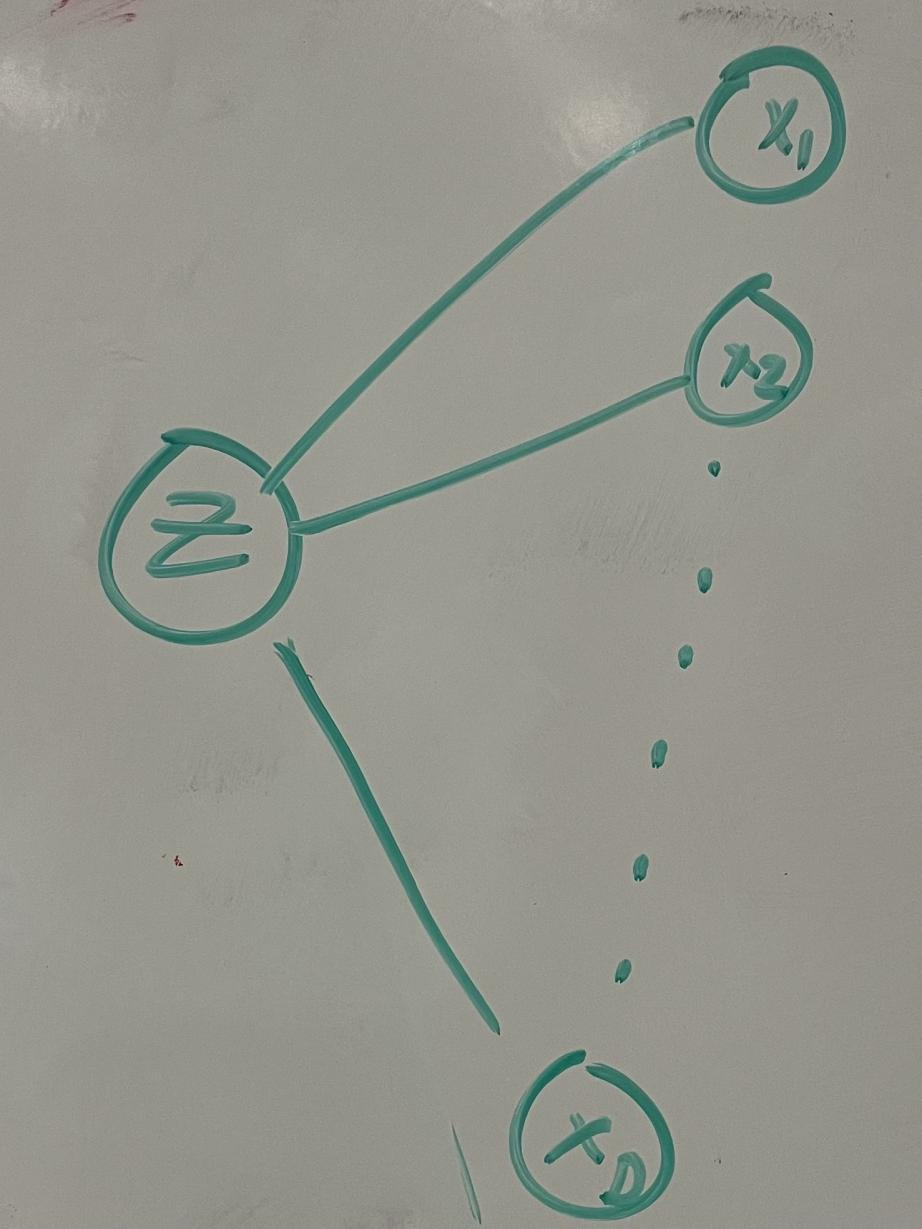
\includegraphics[scale=0.2]{fig1.jpg}
\subsection*{(b)}
$$P(x_1,...,x_D,z)=\boxed{P(z)\Pi_{i=1}^{D}P(x_1|z)}$$
\subsection*{(c)}
Yes they are independent, intuitively thinking for two any two dimensions $x_i$ and $x_j$, this becomes a graphical model with one parent and two children, which was proved in lecture to 
be not independent.

 \section*{Problem 4}
 \subsection*{(a)}

$$P(x_1,x_2,x_3,x_4)=\boxed{P(x_1)P(x_2|x_1)P(x_3|x_2)P(x_4|x_3)}$$
\subsection*{(b)}
for $x_i$ we have
\begin{align*}
    Var(x_i)&=E[x_i^2]-E^2[x_i]\\
    &=E[E[x_i^2|x_{i-1}]]\\
    &=E[\sigma^2+x_{i-1}^2]\\
    &=\sigma^2+E[E[x_{i-1}^2|x_{i-2}]]\\
    &\vdots\\
    &=i\sigma^2
\end{align*}
And for any $i$ and $j$ such that $i<j$
\begin{align*}
    Cov(x_i,x_j)&=E[(x_i-E[x_j])(x_i-E[x_j])]\\
    &=E[x_ix_j]\\
    &=E[E[x_ix_j|x_{j-1}]]\\
    &=E[x_ix_{j-1}]\\
    &\vdots\\
    &=E[x_i^2]\\
    &=i\sigma^2
\end{align*}
Therefore, the covariance matrix $\Sigma$ is
$$\Sigma=\boxed{\begin{bmatrix}
    \sigma^2 & \sigma^2 & \sigma^2 & \sigma^2\\
    \sigma^2 & 2\sigma^2 & 2\sigma^2 & 2\sigma^2\\
    \sigma^2 & 2\sigma^2 & 3\sigma^2 & 3\sigma^2\\
    \sigma^2 & 2\sigma^2 & 3\sigma^2 & 4\sigma^2
    \end{bmatrix}}$$

\subsection*{(c)}
From python the inverse of the precision matrix is 
$$\Sigma^{-1}=\frac{1}{\sigma^2}\boxed{\begin{bmatrix}
    2 & -1 &  0 &  0\\
    -1&  2& -1&  0\\
    0 & -1&  2& -1\\
    0 & 0 & -1 & 1
    \end{bmatrix}}$$
\subsection*{(d)}
The zeros occur only when the nodes have at least one node in between, therefore these nodes are conditionally independent.
\end{document}